\documentclass{article}
\usepackage{amsmath}
\usepackage[english]{babel}
\usepackage{graphicx}
\usepackage{titling}
\usepackage{url}
\usepackage{authblk}
\usepackage{geometry}
\usepackage{xcolor}
\usepackage{hyperref}
\usepackage{listings}
\title{Computer Vision Programming Homework \#2}
\author{2022094093 Kim Dohoon}
\affil{Department of Data Science, Major in Data Science}
\begin{document}
\maketitle

\section*{Original Image}
First, my own image is:  
\begin{figure}[!ht]
    \centering
    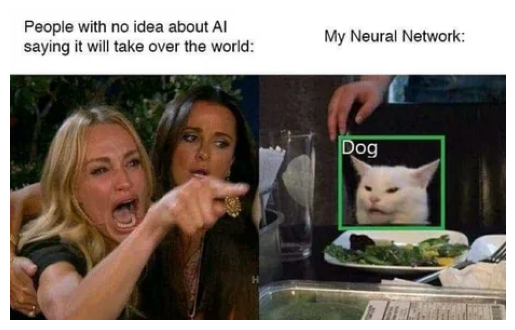
\includegraphics[width=.5\textwidth]{./fig/original.png}
\end{figure}  

which has the resolution $460\times 228$.

Second, the definition of convolution in 2D image is:
$$G[i, j] = \sum_{u=-k}^{k}\sum_{v=-k}^{k}H[u,v]F[i-u,v-j]$$
$$G = H * F$$

\newpage
\section{Mean Filtering}
Gaussian blur, and its standard deviation is 5.

\begin{figure}[!h]
    \centering
    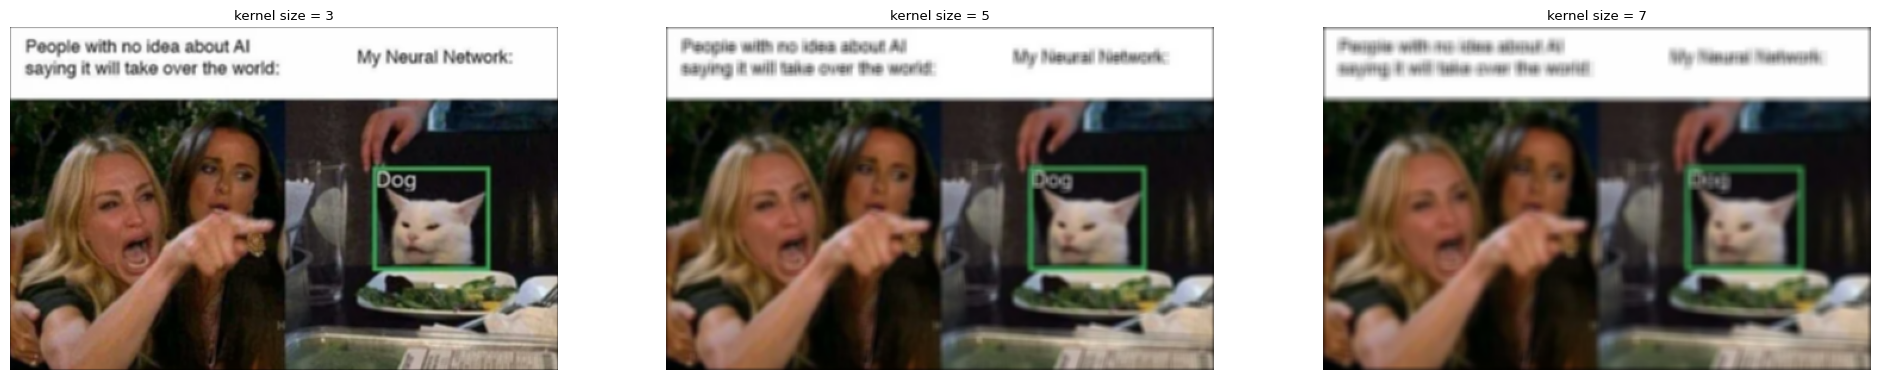
\includegraphics[width=\textwidth]{fig/mean_filtering.png}
    \caption{Gaussian blur with kernel size 3, 5, 7.}
\end{figure}

Also, PSNRs are:
\begin{lstlisting}[backgroundcolor=\color{lightgray}]
kernel=3, PSNR=33.826567540458534
kernel=5, PSNR=32.04943739669039
kernel=7, PSNR=31.195195209214226
\end{lstlisting}

\section{Unsharp Mask}
To implement Unsharp Mask, we can use HPF.
$$\text{HighFrequencyImage} = F + \alpha\cdot(F - F*H)$$
\begin{figure}[!h]
    \centering
    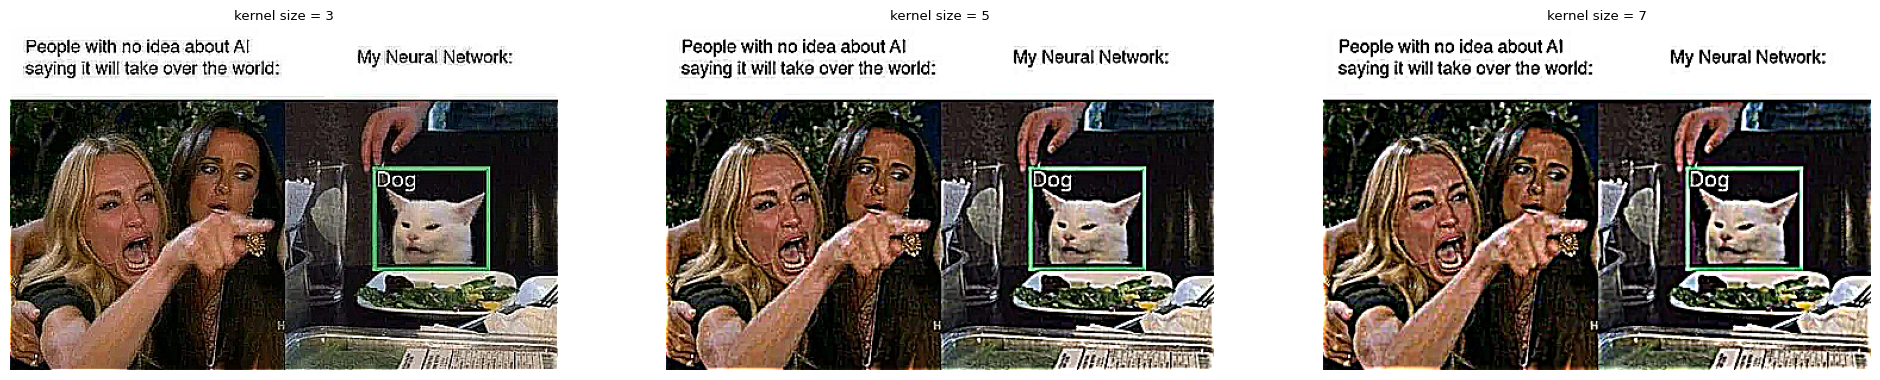
\includegraphics[width=\textwidth]{fig/unsharp_mask.png}
    \caption{Unsharp mask with kernel size 3, 5, 7.}
\end{figure}

\newpage
\section{Contrast Stretching}
First: contrast stretching.
$$v=f(u), u\in[0, 255], v\in[0,255]$$
$$
v = \begin{cases}
    \frac{1}{4}u & 0\leq u < 64 \\
    \frac{7}{4}(u-64)+16 & 64\leq u < 192 \\
    \frac{1}{4}(u-192)+240 & 192\leq u\leq 255 \\
\end{cases}
$$

\begin{figure}[!ht]
    \centering
    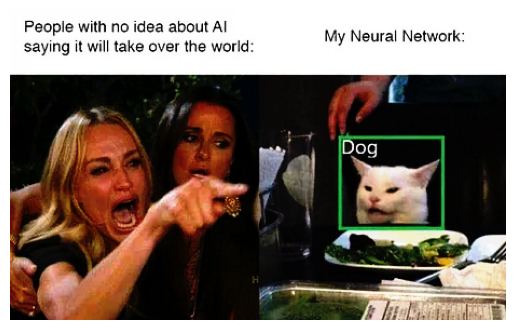
\includegraphics[width=0.5\textwidth]{fig/contrast_stretch.png}
    \caption{Contrast Stretching.}
\end{figure}

Second: gamma correction.
$$v=f(u), u\in[0, 255], v\in[0,255]$$
$$v=1\cdot u^{0.3}$$  

All values are rounded, to make them into integer.
\begin{figure}[!ht]
    \centering
    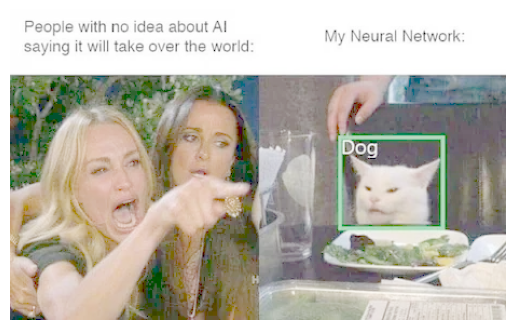
\includegraphics[width=0.5\textwidth]{fig/gamma_corr.png}
    \caption{Gamma Correction.}
\end{figure}

\newpage
\section{Histogram Equalization}
We can use CDF as pixel value, to equalize them.
\begin{figure}[!ht]
    \centering
    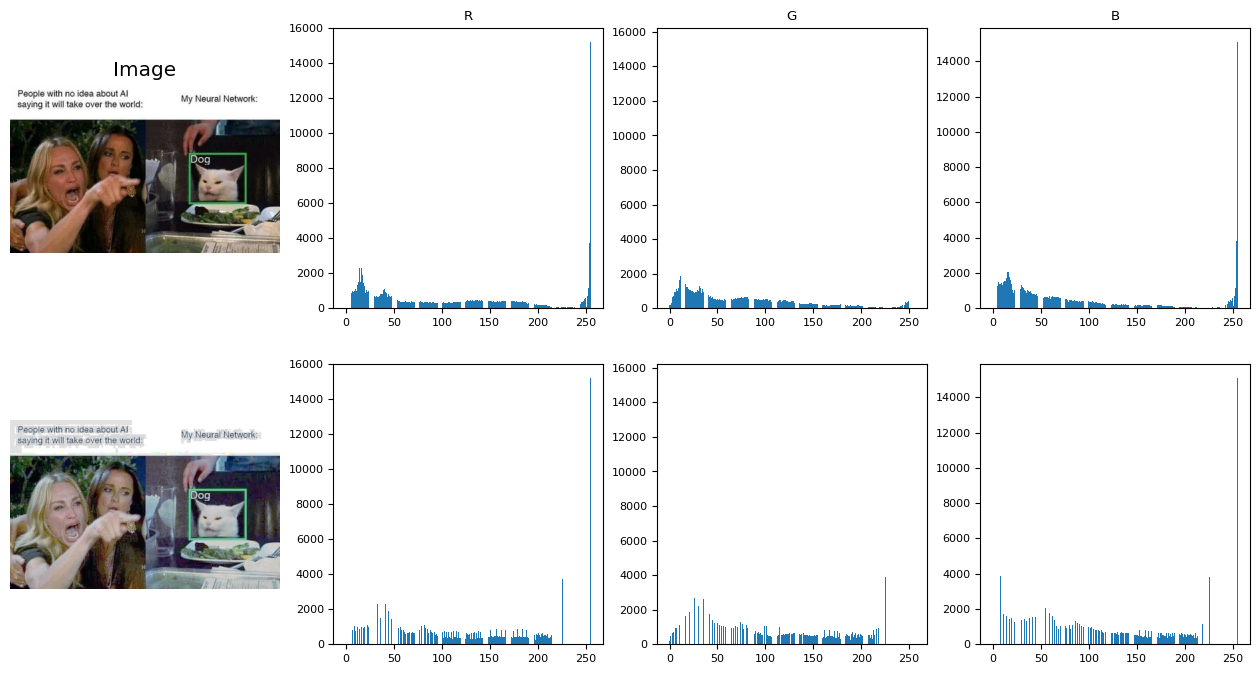
\includegraphics[width=\textwidth]{fig/hist_equalization.png}
    \caption{Histogram Equalization.}
\end{figure}

Upper one is an image before equalization, and lower one is after.

\newpage
\section{Image Upsampling}
After downsampling them, I could get this image.
\begin{figure}[!ht]
    \centering
    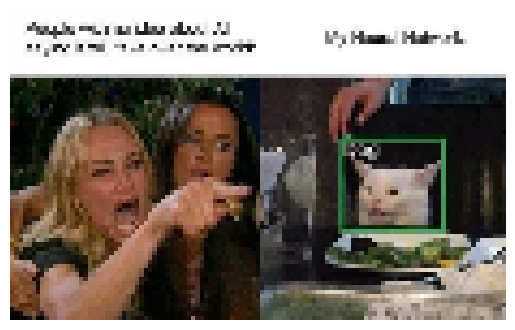
\includegraphics[width=0.5\textwidth]{fig/downsampled.png}
    \caption{Downsampled image. $(460\times 228) \rightarrow (115\times 72)$}
\end{figure}

And three types of interpolation methods are used.
\begin{figure}[!ht]
    \centering
    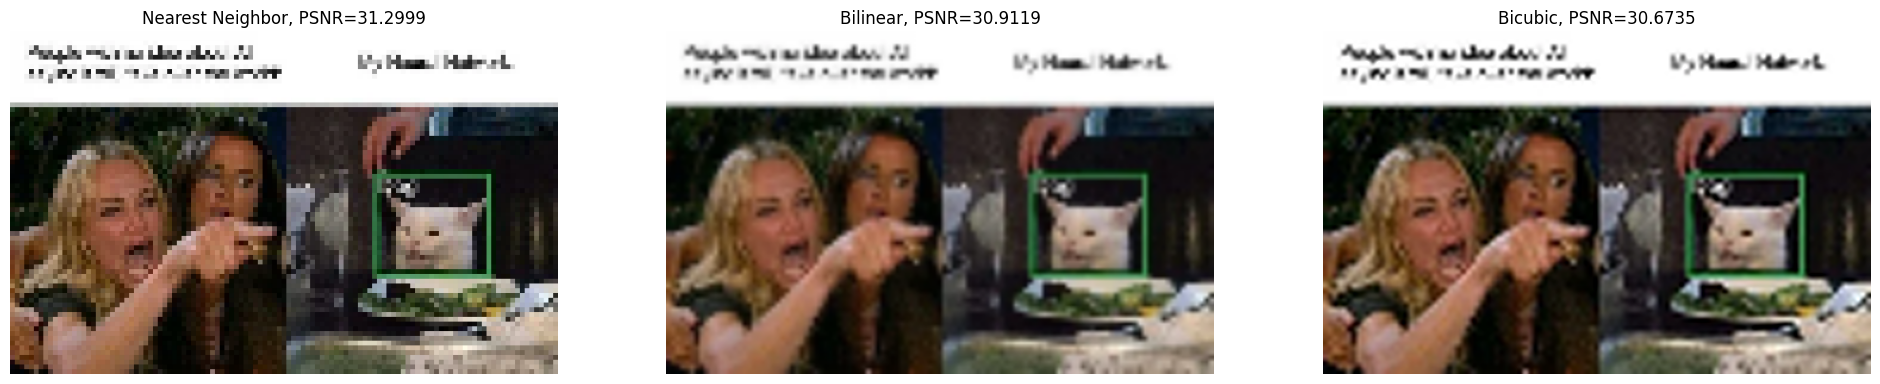
\includegraphics[width=\textwidth]{fig/interpolation.png}
    \caption{After interpolation. Nearest Neightbors, Bilinear, and Bicubic}
\end{figure}

Also, PSNRs are:
\begin{lstlisting}[backgroundcolor=\color{lightgray}]
Nearest Neighbors,  PSNR=31.29986283390819 
Bilinear,           PSNR=30.91187311483395 
Bicubic,            PSNR=30.673464030216874
\end{lstlisting}

\section*{Appendix}
All codes and images are at \url{https://github.com/kdh-yu/ComputerVision/tree/main/HW_2}

\end{document}